
\documentclass[border=10pt, 12pt]{standalone}
\usepackage[svgnames]{xcolor}
\usepackage{amsmath}
\usepackage{pgfplots}
\pgfplotsset{compat=newest}
\usepackage[sfdefault]{FiraSans}
\usepackage{FiraMono}
\renewcommand*\familydefault{\sfdefault}
\begin{document}
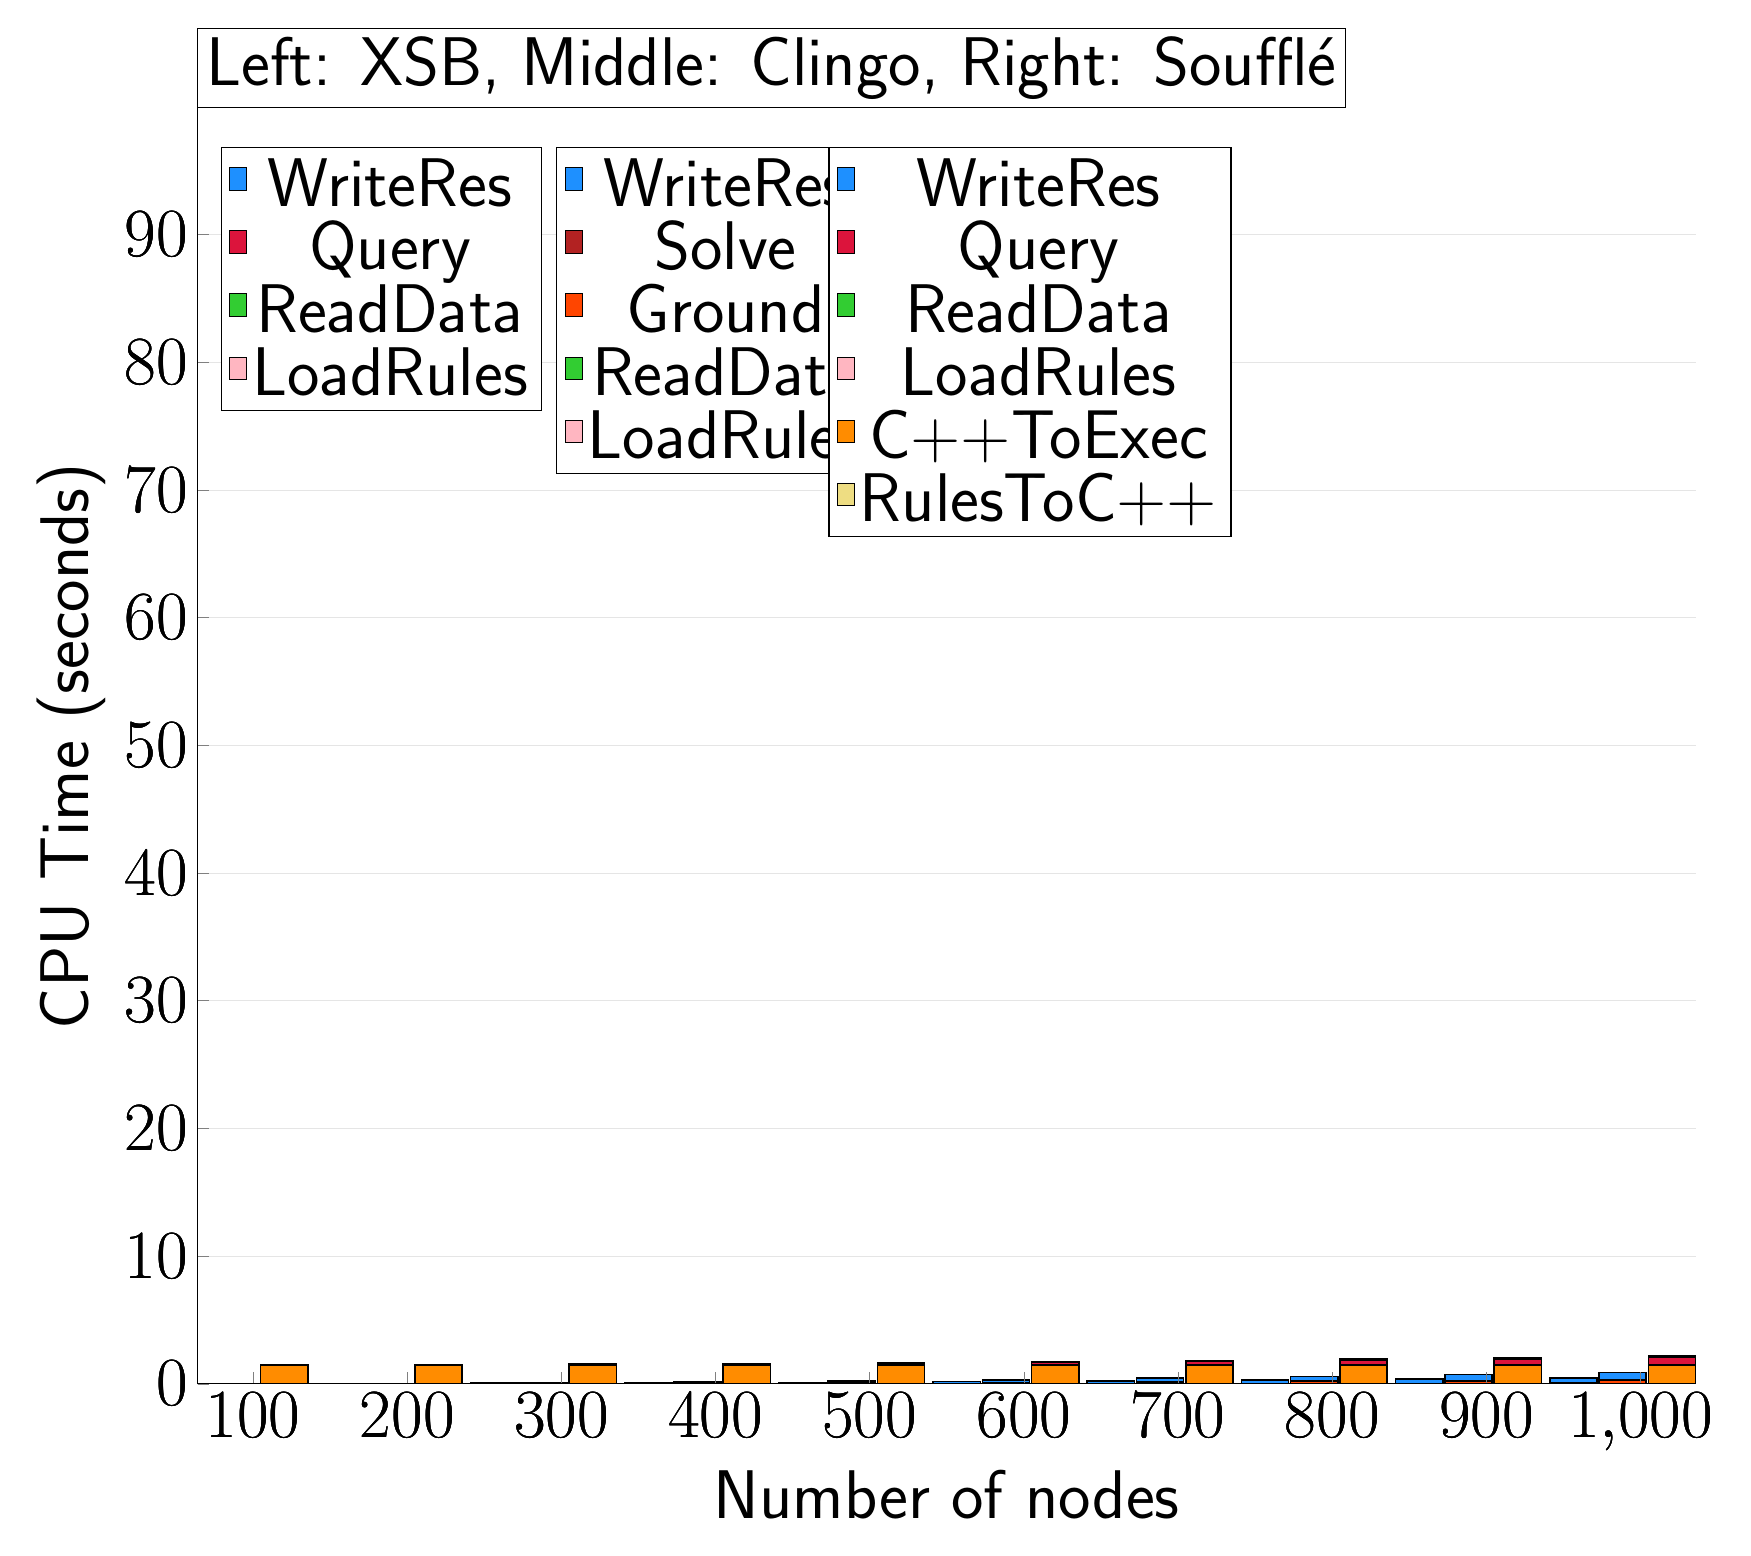
\begin{tikzpicture}
                        \begin{axis}[bar shift=-24.3pt, 
   ybar stacked,
   width=1.7\textwidth,
   bar width=0.6cm,
   ymajorgrids, tick align=inside,
   major grid style={draw=gray!20},
   xtick=data,
   ymin=0, ymax=99.8926,
   axis x line*=bottom,
   axis y line*=left,
   enlarge x limits=0.04,
   legend style={
       at={(0.23, 0.97)},
       anchor=north east,
       legend columns=1,
       font=\Huge,
   },
   ylabel={CPU Time (seconds)},
   xlabel={Number of nodes},
   label style={font=\Huge},
   tick label style={font=\Huge},
]
\addlegendimage{fill=DodgerBlue, draw=black, line width=0.2pt}
\addlegendentry{WriteRes}
\addlegendimage{fill=Crimson, draw=black, line width=0.2pt}
\addlegendentry{Query}
\addlegendimage{fill=LimeGreen, draw=black, line width=0.2pt}
\addlegendentry{ReadData}
\addlegendimage{fill=LightPink, draw=black, line width=0.2pt}
\addlegendentry{LoadRules}
\addplot +[fill=LightPink, draw=black, line width=0.55pt] coordinates {
(100, 0.0005461999999999998)
(200, 0.0005485999999999998)
(300, 0.0005470000000000003)
(400, 0.0005535999999999998)
(500, 0.0005480000000000002)
(600, 0.0005562000000000002)
(700, 0.0005485999999999997)
(800, 0.0005488000000000001)
(900, 0.0005484000000000002)
(1000, 0.0005493999999999995)
};
\addplot +[fill=LimeGreen, draw=black, line width=0.55pt] coordinates {
(100, 0.0001962000000000006)
(200, 0.0002744000000000006)
(300, 0.0003534000000000004)
(400, 0.0004332000000000002)
(500, 0.0005103999999999997)
(600, 0.0005930000000000009)
(700, 0.0006685999999999999)
(800, 0.0007412000000000001)
(900, 0.0008249999999999993)
(1000, 0.0009006)
};
\addplot +[fill=Crimson, draw=black, line width=0.55pt] coordinates {
(100, 0.00042619999999999973)
(200, 0.0017106)
(300, 0.0038436)
(400, 0.007524599999999999)
(500, 0.0121594)
(600, 0.017530200000000003)
(700, 0.023995)
(800, 0.0314694)
(900, 0.040135000000000004)
(1000, 0.050098)
};
\addplot +[fill=DodgerBlue, draw=black, line width=0.55pt] coordinates {
(100, 0.0042134)
(200, 0.0168574)
(300, 0.03817279999999999)
(400, 0.06761179999999999)
(500, 0.1054668)
(600, 0.1525536)
(700, 0.20607440000000002)
(800, 0.2700952)
(900, 0.340826)
(1000, 0.41817779999999993)
};
\end{axis}

\begin{axis}[bar shift=-6.5pt, 
   ybar stacked,
   width=1.7\textwidth,
   bar width=0.6cm,
   ymajorgrids, tick align=inside,
   major grid style={draw=none},
   xtick=data,
   ymin=0, ymax=99.8926,
   axis x line*=none,
   axis y line*=none,
   enlarge x limits=0.04,
   legend style={
       at={(0.454, 0.97)},
       anchor=north east,
       legend columns=1,
       font=\Huge,
   },
   label style={font=\Huge},
   tick label style={font=\Huge},
]
\addlegendimage{fill=DodgerBlue, draw=black, line width=0.2pt}
\addlegendentry{WriteRes}
\addlegendimage{fill=FireBrick, draw=black, line width=0.2pt}
\addlegendentry{Solve}
\addlegendimage{fill=OrangeRed, draw=black, line width=0.2pt}
\addlegendentry{Ground}
\addlegendimage{fill=LimeGreen, draw=black, line width=0.2pt}
\addlegendentry{ReadData}
\addlegendimage{fill=LightPink, draw=black, line width=0.2pt}
\addlegendentry{LoadRules}
\addplot +[fill=LightPink, draw=black, line width=0.55pt] coordinates {
(100, 0.0)
(200, 0.0)
(300, 0.0)
(400, 0.0)
(500, 0.0)
(600, 0.0)
(700, 0.0)
(800, 0.0)
(900, 0.0)
(1000, 0.0)
};
\addplot +[fill=LimeGreen, draw=black, line width=0.55pt] coordinates {
(100, 0.0)
(200, 0.0)
(300, 0.0)
(400, 0.0)
(500, 0.0)
(600, 0.0)
(700, 0.0)
(800, 0.0)
(900, 0.0)
(1000, 0.0)
};
\addplot +[fill=OrangeRed, draw=black, line width=0.55pt] coordinates {
(100, 0.0)
(200, 0.010000000000000009)
(300, 0.020000000000000018)
(400, 0.040000000000000036)
(500, 0.07200000000000001)
(600, 0.10000000000000005)
(700, 0.14200000000000002)
(800, 0.184)
(900, 0.23399999999999999)
(1000, 0.29800000000000004)
};
\addplot +[fill=FireBrick, draw=black, line width=0.55pt] coordinates {
(100, 0.0)
(200, 0.0)
(300, 0.0)
(400, 0.0)
(500, 0.0)
(600, 0.013999999999999974)
(700, 0.018000000000000016)
(800, 0.020000000000000018)
(900, 0.025999999999999995)
(1000, 0.03000000000000001)
};
\addplot +[fill=DodgerBlue, draw=black, line width=0.55pt] coordinates {
(100, 0.008000000000000007)
(200, 0.020000000000000018)
(300, 0.06)
(400, 0.09999999999999998)
(500, 0.16)
(600, 0.20200000000000004)
(700, 0.27999999999999997)
(800, 0.36799999999999994)
(900, 0.4640000000000001)
(1000, 0.5719999999999998)
};
\end{axis}

\begin{axis}[bar shift=11.3pt, 
   ybar stacked,
   width=1.7\textwidth,
   bar width=0.6cm,
   ymajorgrids, tick align=inside,
   major grid style={draw=none},
   xtick=data,
   ymin=0, ymax=99.8926,
   axis x line*=none,
   axis y line*=none,
   enlarge x limits=0.04,
   legend style={
       at={(0.69, 0.97)},
       anchor=north east,
       legend columns=1,
       font=\Huge,
   },
   label style={font=\Huge},
   tick label style={font=\Huge},
]
\addlegendimage{fill=DodgerBlue, draw=black, line width=0.2pt}
\addlegendentry{WriteRes}
\addlegendimage{fill=Crimson, draw=black, line width=0.2pt}
\addlegendentry{Query}
\addlegendimage{fill=LimeGreen, draw=black, line width=0.2pt}
\addlegendentry{ReadData}
\addlegendimage{fill=LightPink, draw=black, line width=0.2pt}
\addlegendentry{LoadRules}
\addlegendimage{fill=DarkOrange, draw=black, line width=0.2pt}
\addlegendentry{C++ToExec}
\addlegendimage{fill=LightGoldenrod, draw=black, line width=0.2pt}
\addlegendentry{RulesToC++}
\addplot +[fill=LightGoldenrod, draw=black, line width=0.55pt] coordinates {
(100, 0.0020000000000000005)
(200, 0.008000000000000002)
(300, 0.006000000000000001)
(400, 0.004000000000000001)
(500, 0.004000000000000001)
(600, 0.0020000000000000005)
(700, 0.0)
(800, 0.004000000000000001)
(900, 0.0020000000000000005)
(1000, 0.0)
};
\addplot +[fill=DarkOrange, draw=black, line width=0.55pt] coordinates {
(100, 1.4659999999999997)
(200, 1.4659999999999997)
(300, 1.472)
(400, 1.474)
(500, 1.472)
(600, 1.4759999999999998)
(700, 1.468)
(800, 1.468)
(900, 1.472)
(1000, 1.472)
};
\addplot +[fill=LightPink, draw=black, line width=0.55pt] coordinates {
(100, 0.00016619999999999997)
(200, 0.0001704)
(300, 0.0001686)
(400, 0.000168)
(500, 0.0001642)
(600, 0.0001656)
(700, 0.00017859999999999998)
(800, 0.00016979999999999998)
(900, 0.0001702)
(1000, 0.00016940000000000002)
};
\addplot +[fill=LimeGreen, draw=black, line width=0.55pt] coordinates {
(100, 0.0007520000000000001)
(200, 0.0012660000000000002)
(300, 0.0016148)
(400, 0.0019364)
(500, 0.0022938)
(600, 0.0027458000000000005)
(700, 0.0029406000000000002)
(800, 0.0034626000000000006)
(900, 0.0036602)
(1000, 0.0040408)
};
\addplot +[fill=Crimson, draw=black, line width=0.55pt] coordinates {
(100, 0.010885200000000001)
(200, 0.037397799999999995)
(300, 0.0684342)
(400, 0.10597920000000001)
(500, 0.15591280000000002)
(600, 0.2180158)
(700, 0.2908906)
(800, 0.3802766)
(900, 0.4780212)
(1000, 0.5967176000000001)
};
\addplot +[fill=DodgerBlue, draw=black, line width=0.55pt] coordinates {
(100, 0.0026088)
(200, 0.006084600000000001)
(300, 0.0102416)
(400, 0.01713)
(500, 0.027051600000000002)
(600, 0.038355)
(700, 0.0524404)
(800, 0.06790840000000001)
(900, 0.085689)
(1000, 0.1066812)
};
\end{axis}


\node[anchor=south, draw, fill=white] at (rel axis cs:0.42,1) {\Huge Left: XSB, Middle: Clingo, Right: Soufflé};
\end{tikzpicture}
\end{document}
                    